% Options for packages loaded elsewhere
\PassOptionsToPackage{unicode}{hyperref}
\PassOptionsToPackage{hyphens}{url}
\PassOptionsToPackage{dvipsnames,svgnames,x11names}{xcolor}
%
\documentclass[
  a4paperpaper,
]{article}

\usepackage{amsmath,amssymb}
\usepackage{iftex}
\ifPDFTeX
  \usepackage[T1]{fontenc}
  \usepackage[utf8]{inputenc}
  \usepackage{textcomp} % provide euro and other symbols
\else % if luatex or xetex
  \ifXeTeX
    \usepackage{mathspec} % this also loads fontspec
  \else
    \usepackage{unicode-math} % this also loads fontspec
  \fi
  \defaultfontfeatures{Scale=MatchLowercase}
  \defaultfontfeatures[\rmfamily]{Ligatures=TeX,Scale=1}
\fi
\usepackage{lmodern}
\ifPDFTeX\else  
    % xetex/luatex font selection
\fi
% Use upquote if available, for straight quotes in verbatim environments
\IfFileExists{upquote.sty}{\usepackage{upquote}}{}
\IfFileExists{microtype.sty}{% use microtype if available
  \usepackage[]{microtype}
  \UseMicrotypeSet[protrusion]{basicmath} % disable protrusion for tt fonts
}{}
\makeatletter
\@ifundefined{KOMAClassName}{% if non-KOMA class
  \IfFileExists{parskip.sty}{%
    \usepackage{parskip}
  }{% else
    \setlength{\parindent}{0pt}
    \setlength{\parskip}{6pt plus 2pt minus 1pt}}
}{% if KOMA class
  \KOMAoptions{parskip=half}}
\makeatother
\usepackage{xcolor}
\setlength{\emergencystretch}{3em} % prevent overfull lines
\setcounter{secnumdepth}{-\maxdimen} % remove section numbering
% Make \paragraph and \subparagraph free-standing
\ifx\paragraph\undefined\else
  \let\oldparagraph\paragraph
  \renewcommand{\paragraph}[1]{\oldparagraph{#1}\mbox{}}
\fi
\ifx\subparagraph\undefined\else
  \let\oldsubparagraph\subparagraph
  \renewcommand{\subparagraph}[1]{\oldsubparagraph{#1}\mbox{}}
\fi

\usepackage{color}
\usepackage{fancyvrb}
\newcommand{\VerbBar}{|}
\newcommand{\VERB}{\Verb[commandchars=\\\{\}]}
\DefineVerbatimEnvironment{Highlighting}{Verbatim}{commandchars=\\\{\}}
% Add ',fontsize=\small' for more characters per line
\usepackage{framed}
\definecolor{shadecolor}{RGB}{241,243,245}
\newenvironment{Shaded}{\begin{snugshade}}{\end{snugshade}}
\newcommand{\AlertTok}[1]{\textcolor[rgb]{0.68,0.00,0.00}{#1}}
\newcommand{\AnnotationTok}[1]{\textcolor[rgb]{0.37,0.37,0.37}{#1}}
\newcommand{\AttributeTok}[1]{\textcolor[rgb]{0.40,0.45,0.13}{#1}}
\newcommand{\BaseNTok}[1]{\textcolor[rgb]{0.68,0.00,0.00}{#1}}
\newcommand{\BuiltInTok}[1]{\textcolor[rgb]{0.00,0.23,0.31}{#1}}
\newcommand{\CharTok}[1]{\textcolor[rgb]{0.13,0.47,0.30}{#1}}
\newcommand{\CommentTok}[1]{\textcolor[rgb]{0.37,0.37,0.37}{#1}}
\newcommand{\CommentVarTok}[1]{\textcolor[rgb]{0.37,0.37,0.37}{\textit{#1}}}
\newcommand{\ConstantTok}[1]{\textcolor[rgb]{0.56,0.35,0.01}{#1}}
\newcommand{\ControlFlowTok}[1]{\textcolor[rgb]{0.00,0.23,0.31}{#1}}
\newcommand{\DataTypeTok}[1]{\textcolor[rgb]{0.68,0.00,0.00}{#1}}
\newcommand{\DecValTok}[1]{\textcolor[rgb]{0.68,0.00,0.00}{#1}}
\newcommand{\DocumentationTok}[1]{\textcolor[rgb]{0.37,0.37,0.37}{\textit{#1}}}
\newcommand{\ErrorTok}[1]{\textcolor[rgb]{0.68,0.00,0.00}{#1}}
\newcommand{\ExtensionTok}[1]{\textcolor[rgb]{0.00,0.23,0.31}{#1}}
\newcommand{\FloatTok}[1]{\textcolor[rgb]{0.68,0.00,0.00}{#1}}
\newcommand{\FunctionTok}[1]{\textcolor[rgb]{0.28,0.35,0.67}{#1}}
\newcommand{\ImportTok}[1]{\textcolor[rgb]{0.00,0.46,0.62}{#1}}
\newcommand{\InformationTok}[1]{\textcolor[rgb]{0.37,0.37,0.37}{#1}}
\newcommand{\KeywordTok}[1]{\textcolor[rgb]{0.00,0.23,0.31}{#1}}
\newcommand{\NormalTok}[1]{\textcolor[rgb]{0.00,0.23,0.31}{#1}}
\newcommand{\OperatorTok}[1]{\textcolor[rgb]{0.37,0.37,0.37}{#1}}
\newcommand{\OtherTok}[1]{\textcolor[rgb]{0.00,0.23,0.31}{#1}}
\newcommand{\PreprocessorTok}[1]{\textcolor[rgb]{0.68,0.00,0.00}{#1}}
\newcommand{\RegionMarkerTok}[1]{\textcolor[rgb]{0.00,0.23,0.31}{#1}}
\newcommand{\SpecialCharTok}[1]{\textcolor[rgb]{0.37,0.37,0.37}{#1}}
\newcommand{\SpecialStringTok}[1]{\textcolor[rgb]{0.13,0.47,0.30}{#1}}
\newcommand{\StringTok}[1]{\textcolor[rgb]{0.13,0.47,0.30}{#1}}
\newcommand{\VariableTok}[1]{\textcolor[rgb]{0.07,0.07,0.07}{#1}}
\newcommand{\VerbatimStringTok}[1]{\textcolor[rgb]{0.13,0.47,0.30}{#1}}
\newcommand{\WarningTok}[1]{\textcolor[rgb]{0.37,0.37,0.37}{\textit{#1}}}

\providecommand{\tightlist}{%
  \setlength{\itemsep}{0pt}\setlength{\parskip}{0pt}}\usepackage{longtable,booktabs,array}
\usepackage{calc} % for calculating minipage widths
% Correct order of tables after \paragraph or \subparagraph
\usepackage{etoolbox}
\makeatletter
\patchcmd\longtable{\par}{\if@noskipsec\mbox{}\fi\par}{}{}
\makeatother
% Allow footnotes in longtable head/foot
\IfFileExists{footnotehyper.sty}{\usepackage{footnotehyper}}{\usepackage{footnote}}
\makesavenoteenv{longtable}
\usepackage{graphicx}
\makeatletter
\def\maxwidth{\ifdim\Gin@nat@width>\linewidth\linewidth\else\Gin@nat@width\fi}
\def\maxheight{\ifdim\Gin@nat@height>\textheight\textheight\else\Gin@nat@height\fi}
\makeatother
% Scale images if necessary, so that they will not overflow the page
% margins by default, and it is still possible to overwrite the defaults
% using explicit options in \includegraphics[width, height, ...]{}
\setkeys{Gin}{width=\maxwidth,height=\maxheight,keepaspectratio}
% Set default figure placement to htbp
\makeatletter
\def\fps@figure{htbp}
\makeatother

\usepackage{fvextra}
\DefineVerbatimEnvironment{Highlighting}{Verbatim}{breaklines,commandchars=\\\{\}}
\DefineVerbatimEnvironment{OutputCode}{Verbatim}{breaklines,commandchars=\\\{\}}
\makeatletter
\@ifpackageloaded{caption}{}{\usepackage{caption}}
\AtBeginDocument{%
\ifdefined\contentsname
  \renewcommand*\contentsname{Índice}
\else
  \newcommand\contentsname{Índice}
\fi
\ifdefined\listfigurename
  \renewcommand*\listfigurename{Lista de Figuras}
\else
  \newcommand\listfigurename{Lista de Figuras}
\fi
\ifdefined\listtablename
  \renewcommand*\listtablename{Lista de Tabelas}
\else
  \newcommand\listtablename{Lista de Tabelas}
\fi
\ifdefined\figurename
  \renewcommand*\figurename{Figura}
\else
  \newcommand\figurename{Figura}
\fi
\ifdefined\tablename
  \renewcommand*\tablename{Tabela}
\else
  \newcommand\tablename{Tabela}
\fi
}
\@ifpackageloaded{float}{}{\usepackage{float}}
\floatstyle{ruled}
\@ifundefined{c@chapter}{\newfloat{codelisting}{h}{lop}}{\newfloat{codelisting}{h}{lop}[chapter]}
\floatname{codelisting}{Listagem}
\newcommand*\listoflistings{\listof{codelisting}{Lista de Listagens}}
\makeatother
\makeatletter
\makeatother
\makeatletter
\@ifpackageloaded{caption}{}{\usepackage{caption}}
\@ifpackageloaded{subcaption}{}{\usepackage{subcaption}}
\makeatother
\ifLuaTeX
\usepackage[bidi=basic]{babel}
\else
\usepackage[bidi=default]{babel}
\fi
\babelprovide[main,import]{portuguese}
% get rid of language-specific shorthands (see #6817):
\let\LanguageShortHands\languageshorthands
\def\languageshorthands#1{}
\ifLuaTeX
  \usepackage{selnolig}  % disable illegal ligatures
\fi
\usepackage{bookmark}

\IfFileExists{xurl.sty}{\usepackage{xurl}}{} % add URL line breaks if available
\urlstyle{same} % disable monospaced font for URLs
\hypersetup{
  pdftitle={Lista 1: Ajustando uma RNA `no braço'},
  pdfauthor={César A. Galvão - 190011572},
  pdflang={pt},
  colorlinks=true,
  linkcolor={blue},
  filecolor={Maroon},
  citecolor={Blue},
  urlcolor={Blue},
  pdfcreator={LaTeX via pandoc}}

\title{Lista 1: Ajustando uma RNA `no braço'}
\author{César A. Galvão - 190011572}
\date{}

\begin{document}
\maketitle

Para essa lista, é considerada a seguinte arquitetura de uma rede neural
\emph{feed-forward}:

\begin{figure}[H]

{\centering 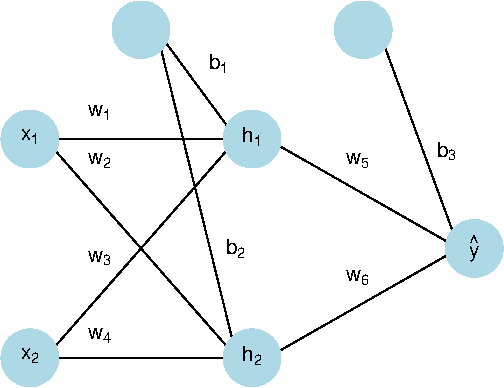
\includegraphics{lista1-resolucao_files/figure-pdf/figf-arquitetura-rede-1.pdf}

}

\caption{Arquitetura da rede neural artificial. Adotamos função de
ativação sigmoide e linear nas camadas escondidas e de saída,
respectivamente.}

\end{figure}%

\section{Questão 1}\label{questuxe3o-1}

\subsection{Item a}\label{item-a}

Crie uma função computacional para calcular o valor previso da variável
resposta \(\hat{y} = f(\boldsymbol{x}; \boldsymbol{\theta})\) em função
de \(\boldsymbol{x}\) e \(\boldsymbol{\theta}\). Use a função para
calcular \(\hat{y}\) para \(\boldsymbol{\theta} = (0.1, \dots , 0.1)\) e
\(\boldsymbol{x} = (1, 1)\).

\begin{center}\rule{0.5\linewidth}{0.5pt}\end{center}

Implementa-se de forma matricial. A função não é adaptativa ao tamanho
da rede e exige que o usuário forneça uma lista \(\boldsymbol{\theta}\)
com os seguintes elementos:

\begin{enumerate}
\def\labelenumi{\arabic{enumi}.}
\tightlist
\item
  \(W^{(1)}\) - matriz \(2 \times 2\) de pesos da camada de entrada
  \(\begin{pmatrix} w_1 & w_2 \\ w_3 & w_4 \end{pmatrix}\). Cada linha
  deve representar os pesos de cada neurônio para o neurônio
  subsequente, i.e.~\(w_{ij}\) representa o peso do neurônio de entrada
  \(i\) para o próximo neurônio \(j\).
\item
  \(\boldsymbol{b}^{(1)}\) - vetor de viés da camada de entrada
  \(\begin{pmatrix} b_1 \\ b_2 \end{pmatrix}\).
\item
  \(W^{(2)}\) - matriz \(2 \times 1\) de pesos da camada de saída
  \(\begin{pmatrix} w_5 \\ w_6 \end{pmatrix}\).
\item
  \(\boldsymbol{b}^{(2)}\) - vetor elemento de viés da camada de saída
  \(\begin{pmatrix} b_3 \end{pmatrix}\).
\end{enumerate}

Como função de ativação foi escolhida a função sigmóide denotada por
\(\phi = \frac{1}{1+e^{-x}}\). A função de previsão é dada por:

\[
\hat{y} = W^{(2)\top}\phi(W^{(1)\top}\boldsymbol{x} + \boldsymbol{b}^{(1)}) + \boldsymbol{b}^{(2)}
\]

ou

\begin{align*}
\boldsymbol{a} =& W^{(1)\top} \boldsymbol{x} + \boldsymbol{b^{(1)}} \\
\boldsymbol{h} =& \phi(\boldsymbol{a}) \\
\hat{y} =& W^{(2)\top}\boldsymbol{h} + b^{(2)}
\end{align*}

\begin{Shaded}
\begin{Highlighting}[]
\CommentTok{\# Função de ativação}
\NormalTok{phi }\OtherTok{\textless{}{-}} \ControlFlowTok{function}\NormalTok{(x) \{}\DecValTok{1}\SpecialCharTok{/}\NormalTok{(}\DecValTok{1} \SpecialCharTok{+} \FunctionTok{exp}\NormalTok{(}\SpecialCharTok{{-}}\NormalTok{x))\}}

\CommentTok{\# Função de previsão}
\NormalTok{ffwd }\OtherTok{\textless{}{-}} \ControlFlowTok{function}\NormalTok{(x, theta) \{}
  
  \ControlFlowTok{if}\NormalTok{(}\FunctionTok{any}\NormalTok{(}\FunctionTok{dim}\NormalTok{(theta[[}\DecValTok{1}\NormalTok{]]) }\SpecialCharTok{!=} \FunctionTok{c}\NormalTok{(}\DecValTok{2}\NormalTok{, }\DecValTok{2}\NormalTok{)))\{}
    \FunctionTok{stop}\NormalTok{(}\StringTok{"Feed Forward: O primeiro elemento de theta deve ser uma matriz de pesos 2x2 para a aplicação nos dados"}\NormalTok{)}
\NormalTok{  \} }\ControlFlowTok{else} \ControlFlowTok{if}\NormalTok{(}\FunctionTok{length}\NormalTok{(theta[[}\DecValTok{2}\NormalTok{]]) }\SpecialCharTok{!=} \DecValTok{2}\NormalTok{)\{}
    \FunctionTok{stop}\NormalTok{(}\StringTok{"Feed Forward: O segundo elemento de theta deve ser um vetor viés de tamanho 2 para somar aos dados"}\NormalTok{)}
\NormalTok{  \} }\ControlFlowTok{else} \ControlFlowTok{if}\NormalTok{(}\FunctionTok{any}\NormalTok{(}\FunctionTok{dim}\NormalTok{(theta[[}\DecValTok{3}\NormalTok{]]) }\SpecialCharTok{!=} \FunctionTok{c}\NormalTok{(}\DecValTok{2}\NormalTok{, }\DecValTok{1}\NormalTok{)))\{}
    \FunctionTok{stop}\NormalTok{(}\StringTok{"Feed Forward: O terceiro elemento de theta deve ser uma matriz de pesos 2x1 para aplicação na única camada h"}\NormalTok{)}
\NormalTok{  \} }\ControlFlowTok{else} \ControlFlowTok{if}\NormalTok{(}\FunctionTok{length}\NormalTok{(theta[[}\DecValTok{4}\NormalTok{]]) }\SpecialCharTok{!=} \DecValTok{1}\NormalTok{)\{}
    \FunctionTok{stop}\NormalTok{(}\StringTok{"Feed Forward: O quarto elemento de theta deve ser um vetor viés de tamanho 1 para soma na única camada h"}\NormalTok{)}
\NormalTok{  \} }\ControlFlowTok{else} \ControlFlowTok{if}\NormalTok{(}\SpecialCharTok{!}\FunctionTok{is.vector}\NormalTok{(x) }\SpecialCharTok{\&} \FunctionTok{length}\NormalTok{(x) }\SpecialCharTok{!=} \DecValTok{2}\NormalTok{)\{}
    \FunctionTok{stop}\NormalTok{(}\StringTok{"Feed Forward: x deve ser um vetor de tamanho 2"}\NormalTok{)}
\NormalTok{  \}}
  
\NormalTok{  x }\OtherTok{\textless{}{-}} \FunctionTok{as.vector}\NormalTok{(x)}
  
\NormalTok{  W1 }\OtherTok{\textless{}{-}}\NormalTok{ theta[[}\DecValTok{1}\NormalTok{]]}
\NormalTok{  b1 }\OtherTok{\textless{}{-}}\NormalTok{ theta[[}\DecValTok{2}\NormalTok{]]}
\NormalTok{  W2 }\OtherTok{\textless{}{-}}\NormalTok{ theta[[}\DecValTok{3}\NormalTok{]]}
\NormalTok{  b2 }\OtherTok{\textless{}{-}}\NormalTok{ theta[[}\DecValTok{4}\NormalTok{]]}
  
\NormalTok{  a }\OtherTok{\textless{}{-}}\NormalTok{ (}\FunctionTok{t}\NormalTok{(W1)}\SpecialCharTok{\%*\%}\NormalTok{x)}\SpecialCharTok{+}\NormalTok{b1}
\NormalTok{  h }\OtherTok{\textless{}{-}} \FunctionTok{phi}\NormalTok{(a)}
\NormalTok{  yhat }\OtherTok{\textless{}{-}}\NormalTok{ (}\FunctionTok{t}\NormalTok{(W2)}\SpecialCharTok{\%*\%}\NormalTok{h)}\SpecialCharTok{+}\NormalTok{b2}
  
  \FunctionTok{return}\NormalTok{( }\CommentTok{\# separacao dos elementos de saída para usar no backpropagation}
    \FunctionTok{list}\NormalTok{(}\AttributeTok{yhat =} \FunctionTok{as.double}\NormalTok{(yhat),}
         \AttributeTok{hidden =}\NormalTok{ h,}
         \AttributeTok{pre\_activation =}\NormalTok{ a)}
\NormalTok{  )}
\NormalTok{\}}
\end{Highlighting}
\end{Shaded}

~

Agora vamos calcular \(\hat{y}\) para
\(\boldsymbol{\theta} = (0.1, \dots , 0.1)\) e
\(\boldsymbol{x} = (1, 1)\).

\begin{Shaded}
\begin{Highlighting}[]
\NormalTok{x }\OtherTok{\textless{}{-}} \FunctionTok{c}\NormalTok{(}\DecValTok{1}\NormalTok{,}\DecValTok{1}\NormalTok{)}

\NormalTok{theta }\OtherTok{\textless{}{-}} \FunctionTok{list}\NormalTok{(}
  \AttributeTok{M1 =} \FunctionTok{matrix}\NormalTok{(}\FunctionTok{c}\NormalTok{(}\FloatTok{0.1}\NormalTok{), }\AttributeTok{nrow =} \DecValTok{2}\NormalTok{, }\AttributeTok{ncol =} \DecValTok{2}\NormalTok{), }
  \AttributeTok{b12 =} \FunctionTok{c}\NormalTok{(}\FloatTok{0.1}\NormalTok{, }\FloatTok{0.1}\NormalTok{), }
  \AttributeTok{M2 =} \FunctionTok{matrix}\NormalTok{(}\FunctionTok{c}\NormalTok{(}\FloatTok{0.1}\NormalTok{), }\AttributeTok{nrow =} \DecValTok{2}\NormalTok{, }\AttributeTok{ncol =} \DecValTok{1}\NormalTok{), }
  \AttributeTok{b3 =} \FunctionTok{c}\NormalTok{(}\FloatTok{0.1}\NormalTok{) }
\NormalTok{)}

\FunctionTok{ffwd}\NormalTok{(x, theta)}
\end{Highlighting}
\end{Shaded}

Obtemos \(\hat{y} =\) 0.2148885.

\subsection{Item b}\label{item-b}

Crie uma rotina computacional para calcular a função de custo
\(J(\theta)\). Em seguida, divida o conjunto de dados observados de modo
que as \textbf{primeiras} \(80.000\) amostras componham o conjunto de
\textbf{treinamento}, as próximas \(10.000\) o de \textbf{validação}, e
as \textbf{últimas} \(10.000\) o de \textbf{teste}. Qual é o custo da
rede no \textbf{conjunto de teste} quando
\(\boldsymbol{\theta} = (0.1, . . . , 0.1)\)?

\begin{center}\rule{0.5\linewidth}{0.5pt}\end{center}

Primeiro são gerados os dados conforme as instruções da lista:

\begin{Shaded}
\begin{Highlighting}[]
\DocumentationTok{\#\#\# Gerando dados "observados"}
\FunctionTok{set.seed}\NormalTok{(}\FloatTok{1.2024}\NormalTok{)}
\NormalTok{m.obs }\OtherTok{\textless{}{-}} \DecValTok{100000}
\NormalTok{dados }\OtherTok{\textless{}{-}} \FunctionTok{tibble}\NormalTok{(}\AttributeTok{x1.obs=}\FunctionTok{runif}\NormalTok{(m.obs, }\SpecialCharTok{{-}}\DecValTok{3}\NormalTok{, }\DecValTok{3}\NormalTok{),}
                \AttributeTok{x2.obs=}\FunctionTok{runif}\NormalTok{(m.obs, }\SpecialCharTok{{-}}\DecValTok{3}\NormalTok{, }\DecValTok{3}\NormalTok{)) }\SpecialCharTok{\%\textgreater{}\%}
         \FunctionTok{mutate}\NormalTok{(}\AttributeTok{mu=}\FunctionTok{abs}\NormalTok{(x1.obs}\SpecialCharTok{\^{}}\DecValTok{3} \SpecialCharTok{{-}} \DecValTok{30}\SpecialCharTok{*}\FunctionTok{sin}\NormalTok{(x2.obs) }\SpecialCharTok{+} \DecValTok{10}\NormalTok{), }
                \AttributeTok{y=}\FunctionTok{rnorm}\NormalTok{(m.obs, }\AttributeTok{mean=}\NormalTok{mu, }\AttributeTok{sd=}\DecValTok{1}\NormalTok{))}
\end{Highlighting}
\end{Shaded}

~

Depois, implementamos a função de custo \(J(\theta)\), que é dada por

\begin{align*}
  J(\boldsymbol{\theta}) =& \frac{1}{m}\sum\limits_{i = 1}^{m} L \left( f(x_{1i}, x_{2i}; \boldsymbol{\theta}), y_i \right) \\ 
  =& \frac{1}{m}\sum\limits_{i = 1}^{m} \left( f(x_{1i}, x_{2i}; \boldsymbol{\theta}) - y_i \right)^2 \\ 
  =& \frac{1}{m}\sum\limits_{i = 1}^{m} \left( \hat{y}_i - y_i \right)^2,
\end{align*}

onde \(m\) é o número de observações.

\begin{Shaded}
\begin{Highlighting}[]
\NormalTok{J.Loss }\OtherTok{\textless{}{-}} \ControlFlowTok{function}\NormalTok{(dados, theta, target)\{}
  
  \ControlFlowTok{if}\NormalTok{(}\SpecialCharTok{!}\FunctionTok{is.data.frame}\NormalTok{(dados) }\SpecialCharTok{|} \SpecialCharTok{!}\FunctionTok{is\_tibble}\NormalTok{(dados))\{}
    \FunctionTok{stop}\NormalTok{(}\StringTok{"Loss: Dados deve ser uma dataframe ou tibble."}\NormalTok{)}
\NormalTok{  \} }\ControlFlowTok{else} \ControlFlowTok{if}\NormalTok{ (}\FunctionTok{dim}\NormalTok{(dados)[}\DecValTok{2}\NormalTok{] }\SpecialCharTok{!=} \DecValTok{2}\NormalTok{)\{}
    \FunctionTok{stop}\NormalTok{(}\StringTok{"Loss: Matriz de dados deve ter 2 colunas."}\NormalTok{)}
\NormalTok{  \} }\ControlFlowTok{else} \ControlFlowTok{if}\NormalTok{ (}\SpecialCharTok{!}\FunctionTok{is.list}\NormalTok{(theta))\{}
    \FunctionTok{stop}\NormalTok{(}\StringTok{"Loss: Theta deve ser uma lista com pesos e viéses."}\NormalTok{)}
\NormalTok{  \} }\ControlFlowTok{else} \ControlFlowTok{if}\NormalTok{ (}\SpecialCharTok{!}\FunctionTok{is.numeric}\NormalTok{(target))\{}
    \FunctionTok{stop}\NormalTok{(}\StringTok{"Loss: Target deve ser um vetor numérico."}\NormalTok{)}
\NormalTok{  \}}
  
\CommentTok{\# aloca memoria para o tamanho dos dados}
\NormalTok{  yhat }\OtherTok{\textless{}{-}} \FunctionTok{double}\NormalTok{(}\FunctionTok{nrow}\NormalTok{(dados))}
  
\CommentTok{\# aloca memoria para os valores pre ativação dos \textquotesingle{}a\textquotesingle{}  }
\NormalTok{  a }\OtherTok{\textless{}{-}} \FunctionTok{matrix}\NormalTok{(}\AttributeTok{nrow =} \FunctionTok{nrow}\NormalTok{(dados), }\AttributeTok{ncol =} \DecValTok{2}\NormalTok{, }\AttributeTok{dimnames =} \FunctionTok{list}\NormalTok{(}\ConstantTok{NULL}\NormalTok{, }\FunctionTok{c}\NormalTok{(}\StringTok{"a1"}\NormalTok{, }\StringTok{"a2"}\NormalTok{)))}

  
\CommentTok{\# transpoe os dados para termos acesso aos vetores de x que serao passados para a primeira camada da rede}
\NormalTok{  tdados }\OtherTok{\textless{}{-}} \FunctionTok{t}\NormalTok{(}\FunctionTok{as.matrix}\NormalTok{(dados))}
  
  \ControlFlowTok{for}\NormalTok{(i }\ControlFlowTok{in} \DecValTok{1}\SpecialCharTok{:}\FunctionTok{ncol}\NormalTok{(tdados))\{}
\NormalTok{    yhat[i] }\OtherTok{\textless{}{-}} \FunctionTok{ffwd}\NormalTok{(tdados[,i], theta)}\SpecialCharTok{$}\NormalTok{yhat}
\NormalTok{    a[i,] }\OtherTok{\textless{}{-}} \FunctionTok{ffwd}\NormalTok{(tdados[,i], theta)}\SpecialCharTok{$}\NormalTok{pre\_activation}
\NormalTok{  \}}
  
  \FunctionTok{return}\NormalTok{(}
    \FunctionTok{list}\NormalTok{(}
      \AttributeTok{loss =} \FunctionTok{mean}\NormalTok{((target }\SpecialCharTok{{-}}\NormalTok{ yhat)}\SpecialCharTok{\^{}}\DecValTok{2}\NormalTok{), }\CommentTok{\#média ja entrega soma/m}
      \AttributeTok{yhat =}\NormalTok{ yhat,}
      \AttributeTok{pre\_activation =}\NormalTok{ a,}
      \AttributeTok{hidden =} \FunctionTok{matrix}\NormalTok{(}\FunctionTok{c}\NormalTok{(}\FunctionTok{phi}\NormalTok{(a[,}\DecValTok{1}\NormalTok{]), }\FunctionTok{phi}\NormalTok{(a[,}\DecValTok{2}\NormalTok{])), }\AttributeTok{ncol =} \DecValTok{2}\NormalTok{)}
\NormalTok{    )}
\NormalTok{  )}
\NormalTok{\}}
\end{Highlighting}
\end{Shaded}

~

Em seguida, separamos o nosso conjunto de dados em treinamento,
validação e teste.

\begin{Shaded}
\begin{Highlighting}[]
\NormalTok{dados\_train }\OtherTok{\textless{}{-}}\NormalTok{ dados[}\DecValTok{1}\SpecialCharTok{:}\DecValTok{80000}\NormalTok{,]}
\NormalTok{dados\_valid }\OtherTok{\textless{}{-}}\NormalTok{ dados[}\DecValTok{80001}\SpecialCharTok{:}\DecValTok{90000}\NormalTok{,]}
\NormalTok{dados\_test }\OtherTok{\textless{}{-}}\NormalTok{ dados[}\DecValTok{90001}\SpecialCharTok{:}\FunctionTok{nrow}\NormalTok{(dados),]}
\end{Highlighting}
\end{Shaded}

~

Finalmente, executamos a função de \emph{feed-forward} nos dados gerados
para calcularmos \(\boldsymbol{\hat{y}}\) e em seguida calculamos o
custo da rede com \(\boldsymbol{\theta} = (0.1, \dots, 0.1)\).

\begin{Shaded}
\begin{Highlighting}[]
\CommentTok{\# transformamos os dados em matriz}
\NormalTok{x\_test }\OtherTok{\textless{}{-}}\NormalTok{ dados\_test }\SpecialCharTok{\%\textgreater{}\%} 
  \FunctionTok{select}\NormalTok{(x1.obs, x2.obs)}

\CommentTok{\# separamos o target}
\NormalTok{y\_test }\OtherTok{\textless{}{-}}\NormalTok{ dados\_test }\SpecialCharTok{\%\textgreater{}\%}
  \FunctionTok{pull}\NormalTok{(y)}

\CommentTok{\# theta já foi gerado e será reaproveitado}
\FunctionTok{J.Loss}\NormalTok{(x\_test, theta, y\_test)}\SpecialCharTok{$}\NormalTok{loss}
\end{Highlighting}
\end{Shaded}

~

Obtemos um custo de 663.1286383.

\subsection{Item c}\label{item-c}

Use a regra da cadeia para encontrar expressões algébricas para o vetor
gradiente

\[
\nabla_{\boldsymbol{\theta}}J(\boldsymbol{\theta}) = \left( \frac{\partial J}{\partial w_1}, \dots, \frac{\partial J}{\partial b_3} \right).
\]

\begin{center}\rule{0.5\linewidth}{0.5pt}\end{center}

Desejamos \(\nabla_{\boldsymbol{\theta}}J(\boldsymbol{\theta})\) tal que

\begin{align}
  \nabla_{\boldsymbol{\theta}}J(\boldsymbol{\theta}) &= \nabla_{\boldsymbol{\theta}} \left[ \frac{1}{m} \sum\limits^m_{i = 1} (y - \hat{y}_i)^2 \right] \nonumber \\
  &= \frac{2}{m} \sum\limits^m_{i = 1} (y - \hat{y}_i) \nabla_{\boldsymbol{\theta}} (y - \hat{y}_i), \quad \text{pois } \hat{y}_i = f(x_{1i}, x_{2i}; \boldsymbol{\theta}) \nonumber \\
  &= \frac{2}{m} \sum\limits^m_{i = 1} (y - \hat{y}_i) (-1) \nabla_{\boldsymbol{\theta}} \hat{y}_i \label{101}
\end{align}

Resolvemos o gradiente, considerando
\(\phi(x) = \sigma(x) = \frac{1}{1+ e^{-x}}\),

\begin{align*}
  \nabla_{\boldsymbol{\theta}} \hat{y}_i &= \nabla_{\boldsymbol{\theta}} \left[ h_{1i} w_5 + h_{2i} w_6 + b_3 \right] \\
  &= \nabla_{\boldsymbol{\theta}} \left[ \phi(a_{1i}) w_5 + \phi(a_{2i}) w_6 + b_3 \right] \\
  &= \nabla_{\boldsymbol{\theta}} \left[ \phi(x_{1i} w_1 + x_{2i} w_3 + b_1) w_5 + \phi(x_{1i} w_2 + x_{2i} w_4 + b_2) w_6 + b_3 \right].
\end{align*}

É imediato que

\begin{align*}
  \frac{\partial \hat{y}_i}{\partial b_3} = 1, \quad \frac{\partial \hat{y}_i}{\partial w_5} = h_{1i}, \quad \frac{\partial \hat{y}_i}{\partial w_6} = h_{2i}.
\end{align*}

Para \(b_j, j \in \{1, 2\}\) resolvemos de forma análoga:

\begin{align*}
\frac{\partial \hat{y}_i}{\partial b_1} &= w_5 \frac{\partial h_1}{\partial b_1} = w_5 \frac{\partial}{\partial b_1} \phi(x_{1i} w_1 + x_{2i} w_3 + b_1) \\  
&= w_5 \frac{\partial}{\partial b_1} \left( \frac{1}{1+ e^{-(x_{1i} w_1 + x_{2i} w_3 + b_1)}} \right) \\  
&= w_5 \frac{(-1) \cdot \frac{\partial}{\partial b_1} \left(1+ e^{-(x_{1i} w_1 + x_{2i} w_3 + b_1)} \right)}{\left(1+ e^{-(x_{1i} w_1 + x_{2i} w_3 + b_1)} \right)^2}
\end{align*}

e

\begin{align*}
\frac{\partial}{\partial b_1} \left(1+ e^{x_{1i} w_1 + x_{2i} w_3 + b_1} \right) &= 1 \cdot e^{x_{1i} w_1 + x_{2i} w_3 + b_1} \\
&= e^{x_{1i} w_1 + x_{2i} w_3 + b_1} = e^{a_1}.
\end{align*}

Portanto,

\begin{align*}
  \frac{\partial \hat{y}_i}{\partial b_1} &= w_5 \frac{-e^{a_1}}{\left( 1+e^{a_1} \right)^2 }, \quad \text{e } \quad \frac{\partial \hat{y}_i}{\partial b_2} = w_6 \frac{-e^{a_2}}{\left( 1+e^{a_2} \right)^2 }.
\end{align*}

Para \(w_j, j \in \{ 1, 2, 3, 4 \}\),

\begin{align*}
  \frac{\partial \hat{y}_i}{\partial w_1} &= w_5 \frac{\partial h_1}{\partial w_1} = w_5 \frac{-x_{1i} \, e^{a_1}}{\left(1 + e^{a_1}\right)^2} \\
  \frac{\partial \hat{y}_i}{\partial w_2} &= w_6 \frac{-x_{1i} \, e^{a_2}}{\left(1 + e^{a_2}\right)^2} \\
  \frac{\partial \hat{y}_i}{\partial w_3} &= w_5 \frac{-x_{2i} \, e^{a_1}}{\left(1 + e^{a_1}\right)^2} \\
  \frac{\partial \hat{y}_i}{\partial w_4} &= w_6 \frac{-x_{2i} \, e^{a_2}}{\left(1 + e^{a_2}\right)^2}.
\end{align*}

Finalmente, substituimos os as componentes na equação (\ref{101}) e
explicitamos cada componente do gradiente\footnote{Essa notação poderia
  ser escrita de forma mais elegante e sucinta. No entanto, dessa forma
  facilita a comparação entre a expressão analítica e a implementação
  computacional pelo leitor.}:

\begin{align}
  \nabla_{\boldsymbol{\theta}}J(\boldsymbol{\theta}) = \begin{pmatrix}
% MATRIZ SIMPLIFICADA
\frac{\partial J}{\partial w_1} \\ \\
\frac{\partial J}{\partial w_2} \\ \\
\frac{\partial J}{\partial w_3} \\ \\
\frac{\partial J}{\partial w_4} \\ \\
\frac{\partial J}{\partial w_5} \\ \\
\frac{\partial J}{\partial w_6} \\ \\
\frac{\partial J}{\partial b_1} \\ \\
\frac{\partial J}{\partial b_2} \\ \\
\frac{\partial J}{\partial b_3} \end{pmatrix} = \begin{pmatrix} 
% MATRIZ EXPLÍCITA
\frac{2}{m} \sum\limits^m_{i = 1}(y - \hat{y}_i) \, w_5 \, x_{1i} \frac{e^{a_{1i}}}{(1+e^{a_{1i}})^2} \\ \\ 
\frac{2}{m} \sum\limits^m_{i = 1}(y - \hat{y}_i) \, w_6 \, x_{1i} \frac{e^{a_{2i}}}{(1+e^{a_{2i}})^2} \\ \\ 
\frac{2}{m} \sum\limits^m_{i = 1}(y - \hat{y}_i) \, w_5 \, x_{2i} \frac{e^{a_{1i}}}{(1+e^{a_{1i}})^2} \\ \\ 
\frac{2}{m} \sum\limits^m_{i = 1}(y - \hat{y}_i) \, w_6 \, x_{2i} \frac{e^{a_{2i}}}{(1+e^{a_{2i}})^2} \\ \\ 
\frac{2}{m} \sum\limits^m_{i = 1}(y - \hat{y}_i) \, (-h_{1i}) \\ \\ 
\frac{2}{m} \sum\limits^m_{i = 1}(y - \hat{y}_i) \, (-h_{2i}) \\ \\ 
\frac{2}{m} \sum\limits^m_{i = 1}(y - \hat{y}_i) \, w_5 \frac{e^{a_{1i}}}{(1+e^{a_{1i}})^2} \\ \\ 
\frac{2}{m} \sum\limits^m_{i = 1}(y - \hat{y}_i) \, w_6 \frac{e^{a_{2i}}}{(1+e^{a_{2i}})^2} \\ \\ 
\frac{2}{m} \sum\limits^m_{i = 1}(y - \hat{y}_i)(-1)
\end{pmatrix} \label{102}
\end{align}  

~

\subsection{Item d}\label{item-d}

Crie uma função computacional que receba como entrada o vetor
\(\theta\), uma matriz design \((x)\) e as respectivas observações
\((y)\) e forneça, como saída, o gradiente definido no item c).
Apresente o resultado da função aplicada sobre o banco de treinamento,
quando \(\theta = (0.1, \dots , 0.1)\). Atenção: implemente o algoritmo
\emph{back-propagation} (Algoritmo 6.4 do livro Deep Learning) para
evitar realizar a mesma operação múltiplas vezes.

\begin{center}\rule{0.5\linewidth}{0.5pt}\end{center}

Primeiramente, implementamos o gradiente encontrado em (\ref{102}):

\begin{Shaded}
\begin{Highlighting}[]
\NormalTok{gradiente }\OtherTok{\textless{}{-}} \ControlFlowTok{function}\NormalTok{(dados, theta, target)\{}
  
  \ControlFlowTok{if}\NormalTok{(}\SpecialCharTok{!}\FunctionTok{is.list}\NormalTok{(theta))\{}
    \FunctionTok{stop}\NormalTok{(}\StringTok{"Gradiente: Theta deve ser uma lista com pesos e viéses."}\NormalTok{)}
\NormalTok{  \} }\ControlFlowTok{else} \ControlFlowTok{if}\NormalTok{(}\SpecialCharTok{!}\FunctionTok{is.data.frame}\NormalTok{(dados) }\SpecialCharTok{|} \SpecialCharTok{!}\FunctionTok{is\_tibble}\NormalTok{(dados))\{}
    \FunctionTok{stop}\NormalTok{(}\StringTok{"Gradiente: Dados deve ser uma dataframe ou tibble."}\NormalTok{)}
\NormalTok{  \} }\ControlFlowTok{else} \ControlFlowTok{if}\NormalTok{(}\SpecialCharTok{!}\FunctionTok{is.numeric}\NormalTok{(target))\{}
    \FunctionTok{stop}\NormalTok{(}\StringTok{"Gradiente: Target deve ser um vetor numérico."}\NormalTok{)}
\NormalTok{  \}}

\NormalTok{  loss\_results }\OtherTok{\textless{}{-}} \FunctionTok{J.Loss}\NormalTok{(dados, theta, target)}
  
  \CommentTok{\# vetor de yhat}
\NormalTok{  yhat }\OtherTok{\textless{}{-}}\NormalTok{ loss\_results}\SpecialCharTok{$}\NormalTok{yhat}
  
  \CommentTok{\# pre\_activation da J.Loss retorna o vetor de \textquotesingle{}a\textquotesingle{}}
\NormalTok{  a }\OtherTok{\textless{}{-}}\NormalTok{ loss\_results}\SpecialCharTok{$}\NormalTok{pre\_activation}
  \CommentTok{\#transformacao em nos neuronios pre{-}ativacao}
\NormalTok{  a}\OtherTok{\textless{}{-}} \FunctionTok{exp}\NormalTok{(a)}\SpecialCharTok{/}\NormalTok{(}\DecValTok{1}\SpecialCharTok{+} \FunctionTok{exp}\NormalTok{(a))}\SpecialCharTok{\^{}}\DecValTok{2}
  
  \CommentTok{\# diferenca entre (target) y e yhat}
\NormalTok{  diff }\OtherTok{\textless{}{-}}\NormalTok{ (target}\SpecialCharTok{{-}}\NormalTok{yhat)}
  
  \CommentTok{\# dados como uma matriz}
\NormalTok{  dados }\OtherTok{\textless{}{-}} \FunctionTok{as.matrix}\NormalTok{(dados)}
  
\NormalTok{  g\_w1 }\OtherTok{\textless{}{-}} \DecValTok{2}\SpecialCharTok{*}\FunctionTok{mean}\NormalTok{(diff}\SpecialCharTok{*}\NormalTok{theta[[}\DecValTok{3}\NormalTok{]][}\DecValTok{1}\NormalTok{]}\SpecialCharTok{*}\NormalTok{dados[,}\DecValTok{1}\NormalTok{]}\SpecialCharTok{*}\NormalTok{a[,}\DecValTok{1}\NormalTok{]) }\CommentTok{\#x1, a1, w5}
\NormalTok{  g\_w2 }\OtherTok{\textless{}{-}} \DecValTok{2}\SpecialCharTok{*}\FunctionTok{mean}\NormalTok{(diff}\SpecialCharTok{*}\NormalTok{theta[[}\DecValTok{3}\NormalTok{]][}\DecValTok{2}\NormalTok{]}\SpecialCharTok{*}\NormalTok{dados[,}\DecValTok{1}\NormalTok{]}\SpecialCharTok{*}\NormalTok{a[,}\DecValTok{2}\NormalTok{]) }\CommentTok{\#x1, a2, w6}
\NormalTok{  g\_w3 }\OtherTok{\textless{}{-}} \DecValTok{2}\SpecialCharTok{*}\FunctionTok{mean}\NormalTok{(diff}\SpecialCharTok{*}\NormalTok{theta[[}\DecValTok{3}\NormalTok{]][}\DecValTok{1}\NormalTok{]}\SpecialCharTok{*}\NormalTok{dados[,}\DecValTok{2}\NormalTok{]}\SpecialCharTok{*}\NormalTok{a[,}\DecValTok{1}\NormalTok{]) }\CommentTok{\#x2, a1, w5}
\NormalTok{  g\_w4 }\OtherTok{\textless{}{-}} \DecValTok{2}\SpecialCharTok{*}\FunctionTok{mean}\NormalTok{(diff}\SpecialCharTok{*}\NormalTok{theta[[}\DecValTok{3}\NormalTok{]][}\DecValTok{2}\NormalTok{]}\SpecialCharTok{*}\NormalTok{dados[,}\DecValTok{2}\NormalTok{]}\SpecialCharTok{*}\NormalTok{a[,}\DecValTok{2}\NormalTok{]) }\CommentTok{\#x2, a2, w6}
\NormalTok{  g\_w5 }\OtherTok{\textless{}{-}} \DecValTok{2}\SpecialCharTok{*}\FunctionTok{mean}\NormalTok{(diff}\SpecialCharTok{*}\NormalTok{(}\SpecialCharTok{{-}}\NormalTok{loss\_results}\SpecialCharTok{$}\NormalTok{hidden[,}\DecValTok{1}\NormalTok{])) }\CommentTok{\#h1}
\NormalTok{  g\_w6 }\OtherTok{\textless{}{-}} \DecValTok{2}\SpecialCharTok{*}\FunctionTok{mean}\NormalTok{(diff}\SpecialCharTok{*}\NormalTok{(}\SpecialCharTok{{-}}\NormalTok{loss\_results}\SpecialCharTok{$}\NormalTok{hidden[,}\DecValTok{2}\NormalTok{])) }\CommentTok{\#h2}
\NormalTok{  g\_b1 }\OtherTok{\textless{}{-}} \DecValTok{2}\SpecialCharTok{*}\FunctionTok{mean}\NormalTok{(diff}\SpecialCharTok{*}\NormalTok{theta[[}\DecValTok{3}\NormalTok{]][}\DecValTok{1}\NormalTok{]}\SpecialCharTok{*}\NormalTok{a[,}\DecValTok{1}\NormalTok{]) }\CommentTok{\#a1, w5}
\NormalTok{  g\_b2 }\OtherTok{\textless{}{-}} \DecValTok{2}\SpecialCharTok{*}\FunctionTok{mean}\NormalTok{(diff}\SpecialCharTok{*}\NormalTok{theta[[}\DecValTok{3}\NormalTok{]][}\DecValTok{2}\NormalTok{]}\SpecialCharTok{*}\NormalTok{a[,}\DecValTok{2}\NormalTok{]) }\CommentTok{\#a2, w6}
\NormalTok{  g\_b3 }\OtherTok{\textless{}{-}} \DecValTok{2}\SpecialCharTok{*}\FunctionTok{mean}\NormalTok{(diff}\SpecialCharTok{*}\NormalTok{(}\SpecialCharTok{{-}}\DecValTok{1}\NormalTok{))}
  
\NormalTok{  grad }\OtherTok{\textless{}{-}} \FunctionTok{c}\NormalTok{(g\_w1, g\_w2, g\_w3, g\_w4, g\_w5, g\_w6, g\_b1, g\_b2, g\_b3)}
  \FunctionTok{names}\NormalTok{(grad) }\OtherTok{\textless{}{-}} \FunctionTok{c}\NormalTok{(}\StringTok{"w1"}\NormalTok{, }\StringTok{"w2"}\NormalTok{, }\StringTok{"w3"}\NormalTok{, }\StringTok{"w4"}\NormalTok{, }\StringTok{"w5"}\NormalTok{, }\StringTok{"w6"}\NormalTok{, }\StringTok{"b1"}\NormalTok{, }\StringTok{"b2"}\NormalTok{, }\StringTok{"b3"}\NormalTok{)}
  

  
  \FunctionTok{return}\NormalTok{(  }
    \FunctionTok{list}\NormalTok{(}\AttributeTok{grad =}\NormalTok{ grad,}
       \AttributeTok{loss\_results =} \FunctionTok{list}\NormalTok{(}
         \AttributeTok{loss =}\NormalTok{ loss\_results}\SpecialCharTok{$}\NormalTok{loss,}
         \AttributeTok{yhat =}\NormalTok{ loss\_results}\SpecialCharTok{$}\NormalTok{yhat,}
         \AttributeTok{hidden =}\NormalTok{ loss\_results}\SpecialCharTok{$}\NormalTok{hidden,}
         \AttributeTok{pre\_activation =}\NormalTok{ loss\_results}\SpecialCharTok{$}\NormalTok{pre\_activation}
\NormalTok{        )}
\NormalTok{       )}
\NormalTok{    )}
\NormalTok{\}}
\end{Highlighting}
\end{Shaded}

~

É apresentado a seguir o resultado da função aplicada sobre o banco de
treinamento, quando \(\theta = (0.1, \dots , 0.1)\):

\begin{Shaded}
\begin{Highlighting}[]
\FunctionTok{gradiente}\NormalTok{(dados\_train[,}\FunctionTok{c}\NormalTok{(}\DecValTok{1}\NormalTok{,}\DecValTok{2}\NormalTok{)], theta, dados\_train}\SpecialCharTok{$}\NormalTok{y)}\SpecialCharTok{$}\NormalTok{grad }\SpecialCharTok{\%\textgreater{}\%}
  \FunctionTok{as\_tibble}\NormalTok{() }\SpecialCharTok{\%\textgreater{}\%}
  \FunctionTok{summarise}\NormalTok{(}\AttributeTok{Componente =} \FunctionTok{c}\NormalTok{(}\StringTok{"w1"}\NormalTok{, }\StringTok{"w2"}\NormalTok{, }\StringTok{"w3"}\NormalTok{, }\StringTok{"w4"}\NormalTok{, }\StringTok{"w5"}\NormalTok{, }\StringTok{"w6"}\NormalTok{, }\StringTok{"b1"}\NormalTok{, }\StringTok{"b2"}\NormalTok{, }\StringTok{"b3"}\NormalTok{),}
         \AttributeTok{Derivada =}\NormalTok{ .}\SpecialCharTok{$}\NormalTok{value) }\SpecialCharTok{\%\textgreater{}\%}
\NormalTok{  knitr}\SpecialCharTok{::}\FunctionTok{kable}\NormalTok{()}
\end{Highlighting}
\end{Shaded}

\begin{longtable}[]{@{}lr@{}}
\toprule\noalign{}
Componente & Derivada \\
\midrule\noalign{}
\endhead
\bottomrule\noalign{}
\endlastfoot
w1 & 0.1767887 \\
w2 & 0.1767887 \\
w3 & -0.6458047 \\
w4 & -0.6458047 \\
w5 & -22.3246918 \\
w6 & -22.3246918 \\
b1 & 1.0732662 \\
b2 & 1.0732662 \\
b3 & -43.4113383 \\
\end{longtable}

\subsection{Item e}\label{item-e}

Aplique o método do gradiente para encontrar os parâmetros que minimizam
a função de custo no \textbf{banco de validação}. Inicie o algoritmo no
ponto \(\theta = (0, \dots , 0)\), use taxa de aprendizagem
\(\epsilon = 0.1\) e rode o algoritmo por 100 iterações. Reporte o menor
custo obtido e indique em qual iteração ele foi observado. Apresente
também o vetor de pesos estimado e comente o resultado.

\begin{center}\rule{0.5\linewidth}{0.5pt}\end{center}

Para a \emph{backpropagation} foi implementada a função a seguir que
funciona em um de dois modos: por número de iterações ou por critério de
aceitação. Neste caso, deve ser fornecido um limiar do valor da função
de custo para que o algoritmo pare.

\begin{Shaded}
\begin{Highlighting}[]
\NormalTok{backpropagation }\OtherTok{\textless{}{-}} \ControlFlowTok{function}\NormalTok{(dados, theta, target, }\AttributeTok{learning\_rate =} \ConstantTok{NULL}\NormalTok{, }\AttributeTok{epochs =} \ConstantTok{NULL}\NormalTok{, }\AttributeTok{acceptance =} \ConstantTok{NULL}\NormalTok{)\{}
  
  \ControlFlowTok{if}\NormalTok{(}\SpecialCharTok{!}\FunctionTok{is.list}\NormalTok{(theta))\{}
    \FunctionTok{stop}\NormalTok{(}\StringTok{"Back propagation: Theta deve ser uma lista com pesos e viéses."}\NormalTok{)}
\NormalTok{  \} }\ControlFlowTok{else} \ControlFlowTok{if}\NormalTok{(}\SpecialCharTok{!}\FunctionTok{is.data.frame}\NormalTok{(dados) }\SpecialCharTok{|} \SpecialCharTok{!}\FunctionTok{is\_tibble}\NormalTok{(dados))\{}
    \FunctionTok{stop}\NormalTok{(}\StringTok{"Back propagation: Dados deve ser uma dataframe ou tibble."}\NormalTok{)}
\NormalTok{  \} }\ControlFlowTok{else} \ControlFlowTok{if}\NormalTok{(}\SpecialCharTok{!}\FunctionTok{is.numeric}\NormalTok{(target))\{}
    \FunctionTok{stop}\NormalTok{(}\StringTok{"Back propagation: Target deve ser um vetor numérico."}\NormalTok{)}
\NormalTok{  \} }\ControlFlowTok{else} \ControlFlowTok{if}\NormalTok{ ((}\SpecialCharTok{!}\FunctionTok{is.null}\NormalTok{(epochs) }\SpecialCharTok{\&} \SpecialCharTok{!}\FunctionTok{is.null}\NormalTok{(acceptance)) }\SpecialCharTok{|}\NormalTok{ (}\FunctionTok{is.null}\NormalTok{(epochs) }\SpecialCharTok{\&} \FunctionTok{is.null}\NormalTok{(acceptance)))\{}
    \FunctionTok{stop}\NormalTok{(}\StringTok{"Back propagation: Escolha se devem ser realizadas iterações programadas ou se o critério de parada será definido por um limite."}\NormalTok{)}
\NormalTok{  \} }\ControlFlowTok{else} \ControlFlowTok{if}\NormalTok{ (}\SpecialCharTok{!}\FunctionTok{is.numeric}\NormalTok{(learning\_rate) }\SpecialCharTok{\&} \SpecialCharTok{!}\FunctionTok{is.null}\NormalTok{(learning\_rate) }\SpecialCharTok{\&}\NormalTok{ learning\_rate }\SpecialCharTok{\textgreater{}} \DecValTok{0}\NormalTok{)\{}
    \FunctionTok{stop}\NormalTok{(}\StringTok{"Back propagation: Learning rate deve ser um número real positivo."}\NormalTok{)}
\NormalTok{  \} }\ControlFlowTok{else} \ControlFlowTok{if}\NormalTok{ (}\SpecialCharTok{!}\FunctionTok{is.integer}\NormalTok{(epochs) }\SpecialCharTok{\&} \SpecialCharTok{!}\FunctionTok{is.null}\NormalTok{(epochs))\{}
    \FunctionTok{stop}\NormalTok{(}\StringTok{"Back propagation: Epochs deve ser um número inteiro positivo."}\NormalTok{)}
\NormalTok{  \}}
  

\CommentTok{\# Se for definido por learning rate}
 \ControlFlowTok{if}\NormalTok{(}\SpecialCharTok{!}\FunctionTok{is.null}\NormalTok{(learning\_rate))\{}
\NormalTok{  loss\_history }\OtherTok{\textless{}{-}} \FunctionTok{numeric}\NormalTok{(epochs)}
\CommentTok{\# initiate loop }
  \ControlFlowTok{for}\NormalTok{(i }\ControlFlowTok{in} \DecValTok{1}\SpecialCharTok{:}\NormalTok{epochs)\{}
    \CommentTok{\#1 forward computation and gradient}
\NormalTok{    grad\_results }\OtherTok{\textless{}{-}} \FunctionTok{gradiente}\NormalTok{(dados, theta, target)}
    \CommentTok{\# disponivel: }
    \DocumentationTok{\#\# gradiente.}
    \DocumentationTok{\#\# loss results: yhat, hidden, pre\_activation}
\NormalTok{    loss\_history[i] }\OtherTok{\textless{}{-}}\NormalTok{ grad\_results}\SpecialCharTok{$}\NormalTok{loss\_results}\SpecialCharTok{$}\NormalTok{loss}
    \CommentTok{\#2 back propagate the gradient}
    \CommentTok{\# novos pesos = theta {-} learning rate * gradiente}
   
\NormalTok{    gradient\_list }\OtherTok{\textless{}{-}} \FunctionTok{list}\NormalTok{(}
      \AttributeTok{W1\_update =} \FunctionTok{matrix}\NormalTok{(grad\_results}\SpecialCharTok{$}\NormalTok{grad[}\DecValTok{1}\SpecialCharTok{:}\DecValTok{4}\NormalTok{], }\AttributeTok{nrow =} \DecValTok{2}\NormalTok{, }\AttributeTok{byrow =} \ConstantTok{TRUE}\NormalTok{),}
      \AttributeTok{b12\_update =}\NormalTok{ grad\_results}\SpecialCharTok{$}\NormalTok{grad[}\DecValTok{7}\SpecialCharTok{:}\DecValTok{8}\NormalTok{],}
      \AttributeTok{W2\_update =} \FunctionTok{matrix}\NormalTok{(grad\_results}\SpecialCharTok{$}\NormalTok{grad[}\DecValTok{5}\SpecialCharTok{:}\DecValTok{6}\NormalTok{], }\AttributeTok{nrow =} \DecValTok{2}\NormalTok{, }\AttributeTok{byrow =} \ConstantTok{TRUE}\NormalTok{),}
      \AttributeTok{b3\_update =}\NormalTok{ grad\_results}\SpecialCharTok{$}\NormalTok{grad[}\DecValTok{9}\NormalTok{]}
\NormalTok{    )}
    
\NormalTok{    theta }\OtherTok{\textless{}{-}} \FunctionTok{list}\NormalTok{( }\CommentTok{\#usaremos o mesmo nome para atualizar no loop}
      \AttributeTok{W1 =}\NormalTok{ theta[[}\DecValTok{1}\NormalTok{]] }\SpecialCharTok{{-}}\NormalTok{ learning\_rate}\SpecialCharTok{*}\NormalTok{gradient\_list}\SpecialCharTok{$}\NormalTok{W1\_update,}
      \AttributeTok{b12 =}\NormalTok{ theta[[}\DecValTok{2}\NormalTok{]] }\SpecialCharTok{{-}}\NormalTok{ learning\_rate}\SpecialCharTok{*}\NormalTok{gradient\_list}\SpecialCharTok{$}\NormalTok{b12\_update,}
      \AttributeTok{W2 =}\NormalTok{ theta[[}\DecValTok{3}\NormalTok{]] }\SpecialCharTok{{-}}\NormalTok{ learning\_rate}\SpecialCharTok{*}\NormalTok{gradient\_list}\SpecialCharTok{$}\NormalTok{W2\_update,}
      \AttributeTok{b3 =}\NormalTok{ theta[[}\DecValTok{4}\NormalTok{]] }\SpecialCharTok{{-}}\NormalTok{ learning\_rate}\SpecialCharTok{*}\NormalTok{gradient\_list}\SpecialCharTok{$}\NormalTok{b3\_update}
\NormalTok{    )}
\NormalTok{  \} }
  \CommentTok{\# outputs: pesos finais e histórico de loss}
  \FunctionTok{return}\NormalTok{(}\FunctionTok{list}\NormalTok{(}
    \AttributeTok{theta =}\NormalTok{ theta,}
    \AttributeTok{loss\_history =}\NormalTok{ loss\_history}
\NormalTok{    )}
\NormalTok{  )}
\NormalTok{ \} }\ControlFlowTok{else} \ControlFlowTok{if}\NormalTok{ (}\SpecialCharTok{!}\FunctionTok{is.null}\NormalTok{(acceptance))\{}
   \CommentTok{\# Se for definido por acceptance}
   
\NormalTok{   i }\OtherTok{\textless{}{-}} \DecValTok{1}
\NormalTok{   loss\_history }\OtherTok{\textless{}{-}} \ConstantTok{Inf}
   
   \ControlFlowTok{while}\NormalTok{(loss\_history[i] }\SpecialCharTok{\textgreater{}}\NormalTok{ acceptance)\{}
     \CommentTok{\#1 forward computation and gradient}
\NormalTok{    grad\_results }\OtherTok{\textless{}{-}} \FunctionTok{gradiente}\NormalTok{(dados, theta, target)}
    \CommentTok{\# disponivel: }
    \DocumentationTok{\#\# gradiente.}
    \DocumentationTok{\#\# loss results: yhat, hidden, pre\_activation}
\NormalTok{    loss\_history[i] }\OtherTok{\textless{}{-}}\NormalTok{ grad\_results}\SpecialCharTok{$}\NormalTok{loss\_results}\SpecialCharTok{$}\NormalTok{loss}
    \CommentTok{\#2 back propagate the gradient}
    \CommentTok{\# novos pesos = theta {-} learning rate * gradiente}
   
\NormalTok{    gradient\_list }\OtherTok{\textless{}{-}} \FunctionTok{list}\NormalTok{(}
      \AttributeTok{W1\_update =} \FunctionTok{matrix}\NormalTok{(grad\_results}\SpecialCharTok{$}\NormalTok{grad[}\DecValTok{1}\SpecialCharTok{:}\DecValTok{4}\NormalTok{], }\AttributeTok{nrow =} \DecValTok{2}\NormalTok{, }\AttributeTok{byrow =} \ConstantTok{TRUE}\NormalTok{),}
      \AttributeTok{b12\_update =}\NormalTok{ grad\_results}\SpecialCharTok{$}\NormalTok{grad[}\DecValTok{7}\SpecialCharTok{:}\DecValTok{8}\NormalTok{],}
      \AttributeTok{W2\_update =} \FunctionTok{matrix}\NormalTok{(grad\_results}\SpecialCharTok{$}\NormalTok{grad[}\DecValTok{5}\SpecialCharTok{:}\DecValTok{6}\NormalTok{], }\AttributeTok{nrow =} \DecValTok{2}\NormalTok{, }\AttributeTok{byrow =} \ConstantTok{TRUE}\NormalTok{),}
      \AttributeTok{b3\_update =}\NormalTok{ grad\_results}\SpecialCharTok{$}\NormalTok{grad[}\DecValTok{9}\NormalTok{]}
\NormalTok{    )}
    
\NormalTok{    theta }\OtherTok{\textless{}{-}} \FunctionTok{list}\NormalTok{( }\CommentTok{\#usaremos o mesmo nome para atualizar no loop}
      \AttributeTok{W1 =}\NormalTok{ theta[[}\DecValTok{1}\NormalTok{]] }\SpecialCharTok{{-}}\NormalTok{ learning\_rate}\SpecialCharTok{*}\NormalTok{gradient\_list}\SpecialCharTok{$}\NormalTok{W1\_update,}
      \AttributeTok{b12 =}\NormalTok{ theta[[}\DecValTok{2}\NormalTok{]] }\SpecialCharTok{{-}}\NormalTok{ learning\_rate}\SpecialCharTok{*}\NormalTok{gradient\_list}\SpecialCharTok{$}\NormalTok{b12\_update,}
      \AttributeTok{W2 =}\NormalTok{ theta[[}\DecValTok{3}\NormalTok{]] }\SpecialCharTok{{-}}\NormalTok{ learning\_rate}\SpecialCharTok{*}\NormalTok{gradient\_list}\SpecialCharTok{$}\NormalTok{W2\_update,}
      \AttributeTok{b3 =}\NormalTok{ theta[[}\DecValTok{4}\NormalTok{]] }\SpecialCharTok{{-}}\NormalTok{ learning\_rate}\SpecialCharTok{*}\NormalTok{gradient\_list}\SpecialCharTok{$}\NormalTok{b3\_update}
\NormalTok{    )}
\NormalTok{    i }\OtherTok{\textless{}{-}}\NormalTok{ i}\SpecialCharTok{+}\DecValTok{1}
\NormalTok{   \}}
   \FunctionTok{return}\NormalTok{(}\FunctionTok{list}\NormalTok{(}
    \AttributeTok{theta =}\NormalTok{ theta,}
    \AttributeTok{loss\_history =}\NormalTok{ loss\_history,}
    \AttributeTok{iterations =}\NormalTok{ i}\DecValTok{{-}1}
\NormalTok{    )}
\NormalTok{   )}
\NormalTok{ \}}
\NormalTok{\}}
\end{Highlighting}
\end{Shaded}

~

A seguir é apresentado o resultado da função aplicada sobre o banco de
validação, quando \(\theta = (0, \dots , 0)\), com taxa de aprendizagem
\(\epsilon = 0.1\) e 100 iterações.

\begin{Shaded}
\begin{Highlighting}[]
\NormalTok{theta }\OtherTok{\textless{}{-}} \FunctionTok{list}\NormalTok{(}
  \AttributeTok{W1 =} \FunctionTok{matrix}\NormalTok{(}\FunctionTok{rep}\NormalTok{(}\DecValTok{0}\NormalTok{, }\DecValTok{4}\NormalTok{), }\AttributeTok{nrow =} \DecValTok{2}\NormalTok{, }\AttributeTok{byrow =} \ConstantTok{TRUE}\NormalTok{),}
  \AttributeTok{b12 =} \FunctionTok{c}\NormalTok{(}\DecValTok{0}\NormalTok{, }\DecValTok{0}\NormalTok{),}
  \AttributeTok{W2 =} \FunctionTok{matrix}\NormalTok{(}\FunctionTok{rep}\NormalTok{(}\DecValTok{0}\NormalTok{, }\DecValTok{2}\NormalTok{), }\AttributeTok{nrow =} \DecValTok{2}\NormalTok{, }\AttributeTok{byrow =} \ConstantTok{TRUE}\NormalTok{),}
  \AttributeTok{b3 =} \DecValTok{0}
\NormalTok{)}

\NormalTok{learning\_rate }\OtherTok{\textless{}{-}}  \FloatTok{0.1}

\NormalTok{epochs }\OtherTok{\textless{}{-}} \DecValTok{100}\NormalTok{L}

\NormalTok{y }\OtherTok{\textless{}{-}}\NormalTok{ dados\_valid}\SpecialCharTok{$}\NormalTok{y}
\NormalTok{x }\OtherTok{\textless{}{-}}\NormalTok{ dados\_valid[,}\FunctionTok{c}\NormalTok{(}\DecValTok{1}\NormalTok{,}\DecValTok{2}\NormalTok{)]}

\NormalTok{back\_validacao }\OtherTok{\textless{}{-}} \FunctionTok{backpropagation}\NormalTok{(x, theta, y, learning\_rate, epochs)}
\end{Highlighting}
\end{Shaded}

~

O menor custo obtido foi 164.8767649 e foi observado na iteração 25.

Um gráfico do histórico de custo é apresentado a seguir:

\begin{figure}[H]

\centering{

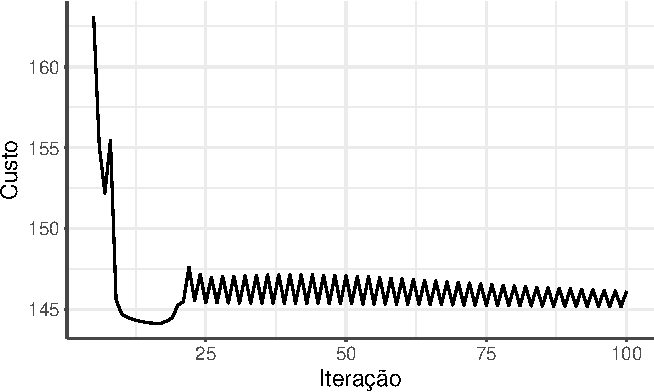
\includegraphics{lista1-resolucao_files/figure-pdf/fig-historico-custo-1.pdf}

}

\caption{\label{fig-historico-custo}Histórico de custo para o banco de
validação.}

\end{figure}%

O vetor de pesos estimado foi:

\begin{align*}
W^{(1)} = \begin{pmatrix} -2.1967097 & -2.1967097 \\ 1.0577389 & 1.0577389 \end{pmatrix}, \quad 
%
\boldsymbol{b}^{(1)} = \begin{pmatrix} -6.8399939 \\ -6.8399939 \end{pmatrix},
\end{align*}

\begin{align*}
W^{(2)} = \begin{pmatrix} -1.0835418 \\ -1.0835418 \end{pmatrix}, \quad 
%
\boldsymbol{b}^{(2)} = 21.8534499.
\end{align*}

Interessantemente, os pesos de cada variavel para a camada seguinte,
assim como os viéses, são idênticos. Além disso, os pesos aplicados nos
neurônios da camada escondida também são idênticos. Isso pode ser um
indicativo de que ambas as variáveis explicativas possuem importância
igual para a previsão da variável resposta. Ao mesmo tempo, ambas
\(X_1\) e \(X_2\) têm o mesmo processo gerador, então não parece ser
surpreendente que os pesos sejam iguais.

Finalmente, o gráfico indica que possivelmente o algoritmo estacionou em
um mínimo local de valor superior ao mínimo encontrado na iteração de
número 25.

\subsection{Item f}\label{item-f}

\section{Lições aprendidas}\label{liuxe7uxf5es-aprendidas}

É muito positivo construir funções que retornam listas com os resultados
de cada etapa do algoritmo. Isso facilita a depuração e a compreensão do
código. Além disso, é importante testar cada função separadamente para
garantir que ela está retornando o resultado esperado.

Frequentemente quando avançava um item, percebia que poderia incrementar
funções anteriores que já retornavam internamente vetores que seriam
usados futuramente. Dessa forma, é possível utilizar listas para fazer
referencias fáceis a componentes de cada etapa e evitar repetições
desnecessárias de cálculos, reduzindo o custo computacional da lista
como um todo.



\end{document}
